\documentclass[a4paper, notitlepage, 10pt]{article}
\usepackage{geometry}
% WSC 2015 configs
\fontfamily{times}
\geometry{verbose,tmargin=30mm,bmargin=25mm,lmargin=25mm,rmargin=25mm}
\pagestyle{empty}
% end configs
\usepackage{setspace,relsize}               
\usepackage{moreverb}                        
\usepackage{url}
\usepackage{hyperref}
\hypersetup{colorlinks=true,citecolor=blue}
\usepackage{amsmath}
\usepackage{mathtools} 
\usepackage{amsthm}
\usepackage{amssymb}
\usepackage{indentfirst}
\usepackage{todonotes}
\usepackage[authoryear,round]{natbib}
\bibliographystyle{apalike}
\usepackage[pdftex]{lscape}
\usepackage[utf8]{inputenc}

% Title Page
\title{\vspace{-9ex}\centering \bf Transform then pool or pool and then transform?}
\author{
Luiz Max F. de Carvalho\\
% Program for Scientific Computing (PROCC), Oswaldo Cruz Foundation. \\
% Institute of Evolutionary Biology, University of Edinburgh.\\
}
\DeclareMathOperator*{\argmin}{arg\,min}
\DeclareMathOperator*{\argmax}{arg\,max}
\newtheorem{theo}{Theorem}[]
\newtheorem{proposition}{Proposition}[]
\newtheorem{remark}{Remark}[]
\newtheorem{definition}{Definition}[]
\setcounter{theo}{0} % assign desired value to theorem counter
\begin{document}
\maketitle

\begin{abstract}
In this note I claim to give a proof that the order of operations between transforming and pooling a set of distributions does not matter~\textbf{if and only if} the transform in question is invertible.
I also give an example where the transform-then-pool and pool-then-transform with a non-invertible transform lead to distributions in the same family which are nonetheless distinct.


Key-words: logarithmic pooling; invertible; log-normal. 
\end{abstract}

\section*{Background}

Logarithmic pooling is a popular method for combining opinions on an agreed quantity, specially when these opinions can be framed as probability distributions.
Let $\mathbf{F_\theta} := \{f_0(\theta), f_1(\theta), \ldots, f_K(\theta)\}$ be a set of distributions representing the opinions of $K + 1$ experts and let $\boldsymbol\alpha :=\{\alpha_0, \alpha_1, \ldots, \alpha_K \} \in \mathcal{S}^K$ be the vector of weights, such that $\alpha_i > 0\: \forall i$ and $\sum_{i=0}^K \alpha_i = 1$, i.e., $\mathcal{S}^{K + 1}$ is the space of all open simplices of dimension $K + 1$.
The \textbf{logarithmic pooling operator} $\mathcal{LP}(\mathbf{F_\theta}, \boldsymbol\alpha)$ is defined as
\begin{equation}
\label{eq:logpool}
 \mathcal{LP}(\mathbf{F_\theta}, \boldsymbol\alpha) :=  \pi(\theta | \boldsymbol\alpha) = t(\boldsymbol\alpha) \prod_{i=0}^K f_i(\theta)^{\alpha_i},
\end{equation}
where $t(\boldsymbol\alpha) = \int_{\boldsymbol\Theta}\prod_{i=0}^K f_i(\theta)^{\alpha_i}d\theta$.
This pooling method enjoys several desirable properties and yields tractable distributions for a large class of distribution families~\citep{genest1984}.

\section*{Pool then transform or transform and then pool?}

\begin{definition}
Let $A, B \subseteq \mathbb{R}^p$.
A function  $h: A \to B$ is \textbf{invertible} iff $\: \exists \: h^{-1}: B \to A \: \text{with} \: h^{-1}(h(a)) = a \: \forall \: a \in A$. 
Let $\pi_A$ be an arbitrary probability measure in A. 
If $h$ is monotonic and differentiable we can write $\pi_B(B) = \pi(h^{-1}(A))|J|$, where $|J|$ is the absolute determinant of the Jacobian matrix with entries $J_{ik} := \partial h_k^{-1}/\partial a_i$, $i,k = 1, 2, \ldots, p$.
\end{definition}

Suppose the we are interested in the distribution of a random variable $Y \in \mathcal{Y}\subseteq \mathbb{R}^q$  when one has a random variable $X \in \mathcal{X} \subseteq \mathbb{R}^p$ with $\phi : \mathcal{X} \to \mathcal{Y}$.
Let $|J_\phi|$ be the Jacobian determinant w.r.t. $\phi$.
Suppose further that each expert $i$ produces a distribution $f_i(X)$ such that we can construct the object $\mathbf{F}_X = \{f_1(X), f_2(X), \ldots, f_K(X) \}$.
Then one can either:
\begin{itemize}
 \item[(a)] \textbf{Pool-then-transform:} construct $\pi_X(X | \boldsymbol \alpha) = \mathcal{LP}(\mathbf{F}_X, \boldsymbol \alpha)$ and then apply $\phi$ to obtain $\pi_Y(Y | \boldsymbol \alpha) := \pi_X( \phi^{-1}(Y)| \boldsymbol\alpha) |J_\phi|$;
 \item[(b)] \textbf{Transform-then-pool:} apply the transform to each component $i$ of $\mathbf{F}_X$ to build
 \[\mathbf{G}_{Y}:= \{g_i(Y), g_2(Y), \ldots, g_K(Y)\} \]
 and obtain $\pi_Y^{\prime}(Y |  \boldsymbol \alpha) = \mathcal{LP}(\mathbf{G}_{Y},  \boldsymbol \alpha)$.
\end{itemize}

\begin{remark}
\label{rmk:invariance}
If $\phi$ is invertible, then $\pi_Y(Y | \boldsymbol \alpha) \equiv \pi_Y^{\prime}(Y|  \boldsymbol \alpha)$.
\end{remark}
\begin{proof}
First, 
\begin{align}
 \pi_Y(y | \boldsymbol \alpha) & \propto \pi_{X}(\phi^{-1}(y))|J_\phi|, \\
&= \prod_{i = 0}^K \left[ f_i(\phi^{-1}(y)) \right]^{\alpha_i}|J_\phi|.
\end{align}
For situation (b) we have:
\begin{equation}
 g_i(y) = f_i(\phi^{-1}(y))|J_\phi|.
\end{equation}
And,
\begin{align}
 \pi_Y^{\prime}(y |  \boldsymbol \alpha) & \propto  \prod_{i=0}^K g_i(y)^{\alpha_i} \\
  & =  \prod_{i=0}^K \left[ f_i(\phi_x^{-1}(y))|J_\phi| \right]^{\alpha_i} \\
  & = \prod_{i = 0}^K \left[ f_i(\phi^{-1}(y)) \right]^{\alpha_i}|J_\phi|,
\end{align}
as claimed.
\end{proof}

An interesting idea is whether Remark~\ref{rmk:invariance} is an iff result. 
Let $\eta : \mathcal{X} \to \mathcal{Y}$ be a surjective non-injective differentiable function, which is not invertible on the whole of $\mathcal{Y}$, but instead is \textbf{piece-wise invertible}.
Let $\mathcal{Y}_1, \mathcal{Y}_2, \ldots, \mathcal{Y}_T$ be a  partition of $\mathcal{Y}$, i.e., $\mathcal{Y}_i\cap\mathcal{Y}_j = \emptyset,\: \forall i\neq j \in \{1, 2, \ldots, T\}$ and $\bigcup_{t = 1}^T\mathcal{Y}_t = \mathcal{Y}$.
Then define the inverse functions $\eta_{t}^{-1}(y)\,:\, \mathcal{Y}_t \to \mathcal{X}, \: t \in \{1, 2, \ldots, T\}$.
Lastly, let $|J_t|$ be the Jacobian of $\eta_{t}^{-1}(\cdot)$.
Then we are prepared to write:
\begin{align}
\label{eq:piecewiseTransf}
\pi_{Y}(y |\boldsymbol\alpha) &\propto \sum_{t = 1}^T\left(\prod_{i=0}^K f_i(\eta_t^{-1}(y))^{\alpha_i}\right)|J_t| \quad \text{and}\\
\pi^{\prime}_{Y}(y|\boldsymbol\alpha) &\propto \prod_{i=0}^K\left[\sum_{t = 1}^T f_i(\eta_t^{-1}(y))|J_t|\right]^{\alpha_i}
\end{align}
which, I claim, will only be equal if $T = 1$, i.e. if $\eta(\cdot)$ is invertible in the usual sense.
Below I try to establish a result in general for any surjective non-injective mapping, not just piece-wise invertible ones.
\begin{remark}
 \label{rmk:invertibleIFF}
 $\pi_Y(Y | \boldsymbol \alpha) \equiv \pi_Y^{\prime}(Y|  \boldsymbol \alpha)$ if and only if $\phi$ is invertible.
\end{remark}
\begin{proof}
 In general, we can define $\Omega(y) := \{ x: \eta(x) = y \}$ and thus\footnote{Notice there is no guarantee that $|\Omega(y)| < \infty$.} 
\begin{equation}
 g_i(y) = \sum_{x \in \Omega(y)} f_i(x).
\end{equation}
Notice that for any $x \in \mathcal{X}$, there exists $y$ and $\Omega(y)$ such that $x \in \Omega(y)$. 
Assume $|\Omega(y)| > 1$ for some $y \in \mathcal{Y}$ and $f_i \not\equiv f_j,$ for some $i, j$.
We have
\begin{align}
\label{eq:generalTransf}
\pi_{Y}(y |\boldsymbol\alpha) &\propto \sum_{x \in \Omega(y)}\left(\prod_{i=0}^K f_i(x)^{\alpha_i}\right) \quad \text{and}\\
\pi^{\prime}_{Y}(y|\boldsymbol\alpha) &\propto \prod_{i=0}^K\left[\sum_{x \in \Omega(y)} f_i(x)\right]^{\alpha_i}.
\end{align}
Define 
\begin{equation*}
 T = \int_{\mathcal{Y}} \sum_{x \in \Omega(y)}\left(\prod_{i=0}^K f_i(x)^{\alpha_i}\right)dy \quad \text{and} \quad T^{\prime}= \int_{\mathcal{Y}} \prod_{i=0}^K\left[\sum_{x \in \Omega(y)} f_i(x)\right]^{\alpha_i} dy.
\end{equation*}
It is not hard to show\footnote{This hinges on the fact that $\int_{\mathcal{Y}} g_i(y) dy = 1 \: \forall \: i$ .} that $T = \left(\int_{\mathcal{X}} \prod_{i=0}^K f_i(x)^{\alpha_i} dx\right)^{-1}$.
Since for any given $y$ and $x \in \Omega(y)$ we have $\sum_{\omega \in \Omega(y)} f_i(\omega) > f_i(x)$~\textit{a.e.}, it follows that $T^\prime < T$ and hence the densities would have different normalising constants, which is impossible if $\pi_{Y}(y |\boldsymbol\alpha) = \pi_{Y}^\prime(y |\boldsymbol\alpha) \: \forall \: y \: \in \mathcal{Y}$.
\end{proof}
There probably exists a measure-theoretic proof that is way more elegant, but this should suffice.

\section*{An example}

Suppose $Z = U/V$ and each expert $i$ elicits $U \sim \text{log-normal}(\mu_{iU}, \sigma_{iU}^2)$, $V \sim \text{log-normal}(\mu_{iV}, \sigma_{iV}^2)$, i.e.
\begin{eqnarray*}
\nonumber
f_{iU}(u | \mu_{iU}, \sigma_{iU}^2) &=& \frac{1}{u \sqrt{2\pi\sigma_{iU}^2}} \exp\left( - \frac{ \left( \ln u - \mu_{iU} \right)^2 }{2 \sigma_{iU}^2} \right), \\
g_{iV}(v | \mu_{iV}, \sigma_{iV}^2) &=& \frac{1}{v \sqrt{2\pi\sigma_{iV}^2}} \exp\left( - \frac{ \left( \ln v - \mu_{iV} \right)^2 }{2 \sigma_{iV}^2} \right).
\end{eqnarray*}
Again, let $\mathbf{F}_U = \{f_{1U}(U), f_{2U}(U), \ldots, f_{KU}(U) \}$ and $\mathbf{G}_V = \{g_{1V}(V), g_{2V}(V), \ldots, g_{KV}(V) \}$.
First, let us derive $\pi_Z(Z)$ under scheme (a).
It is not hard to show that  $\pi_U(U | \boldsymbol\alpha) := \mathcal{LP}(\mathbf{F}_{U}, \boldsymbol \alpha) =  \text{log-normal}(\mu_U^\ast, v_U^\ast)$ with
\begin{align}
 \mu_U^\ast &:= \frac{\sum_{i=0}^K w_{iU} \mu_{iU}}{\sum_{i=0}^K w_{iU}}, \\
 v_U^\ast &:= \frac{1}{\sum_{i=0}^K w_{iU} }, \\
 w_{iU} &:=  \frac{\alpha_i}{\sigma_{iU}^2}.
\end{align}
See our paper for a proof.
Analagously, $\pi_V(V | \boldsymbol\alpha) := \mathcal{LP}(\mathbf{G}_{V}, \boldsymbol \alpha) =  \text{log-normal}(\mu_V^\ast, v_V^\ast)$.
Then $\pi_Z(Z |  \boldsymbol \alpha) = \text{log-normal}(\mu_Z^{\ast}, v_Z^{\ast})$, with
\begin{align}
\nonumber
 \mu_Z^{\ast} &= \mu_U^\ast - \mu_V^\ast,\\
 &= \frac{\sum_{i=0}^K w_{iU} \mu_{iU}}{\sum_{i=0}^K w_{iU}} - \frac{\sum_{i=0}^K w_{iV} \mu_{iV}}{\sum_{i=0}^K w_{iV}}\quad \text{and} \\
 \nonumber
v_Z^{\ast} &= v_U^\ast + v_V^\ast, \\
&= \frac{1}{\sum_{i=0}^K w_{iU} } + \frac{1}{\sum_{i=0}^K w_{iV} }.
\end{align}
Now let us consider case (b).
Since $r_{iZ} = \text{log-normal}(\mu_{iU} - \mu_{iV}, \sigma_{iU}^2 +  \sigma_{iV}^2)$, we arrive at  $\pi_Z^{\prime}(Z |  \boldsymbol \alpha) = \text{log-normal}(\mu_Z^{\ast\ast}, v_Z^{\ast\ast})$,
\begin{align}
 \mu_Z^{\ast\ast} &:= \frac{\sum_{i=0}^K w_{iZ} \mu_{iU}}{\sum_{i=0}^K w_{iZ}} - \frac{\sum_{i=0}^K w_{iZ} \mu_{iV}}{\sum_{i=0}^K w_{iZ}}, \\
 v_Z^{\ast\ast} &:= \frac{1}{\sum_{i=0}^K w_{iZ} }, \\
 w_{iZ} &:=  \frac{\alpha_i}{\sigma_{iU}^2 + \sigma_{iV}^2}.
\end{align}
Clearly, $v_Z^{\ast} \leq v_Z^{\ast\ast}$ and hence $\mu_Z^{\ast\ast} \leq \mu_Z^{\ast} \: \forall \: \boldsymbol\alpha$.

\begin{figure}[!ht]
\centering
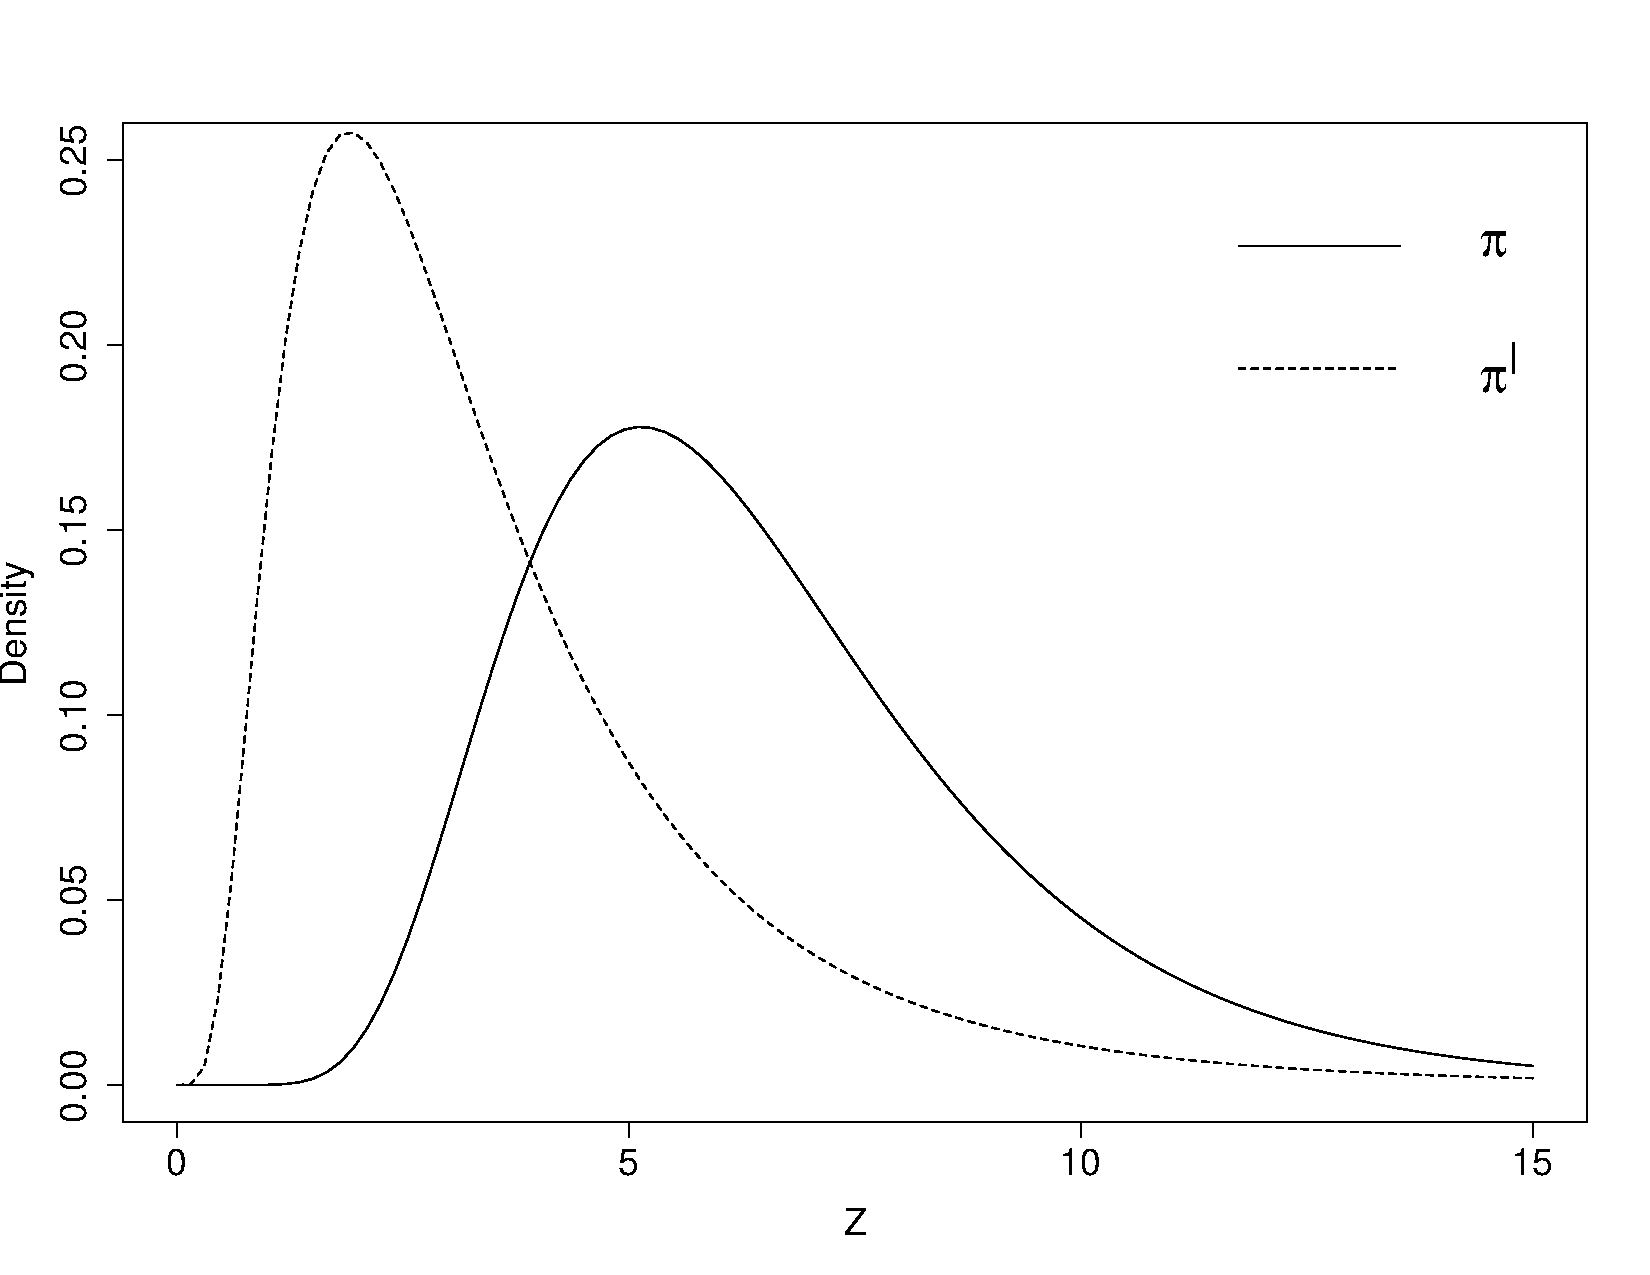
\includegraphics[scale=0.5]{figures/lognormal_example.pdf}
\caption{\textbf{Log-normal example}. Solid line displays $\pi_Z(Z | \boldsymbol\alpha)$, obtained by first pooling the distributions on $U$ and $V$ and then computing the induced distribution on $Z$.
Dashed line displays the logarithmic pooling of individual distributions $r_{iZ}$, $\pi_Z^{\prime}(Z | \boldsymbol\alpha)$.
For this example $K=2$, $\alpha_0 = 0.70$, $\mu_{0U} = 0.80$, $\sigma_{0U}^2 = 0.40$, $\mu_{1U} = 0.5$, $\sigma_{1U}^2 = 0.05$, $\mu_{0V} = -1.60$, $\sigma_{0V}^2 = 0.024$, $\mu_{1V} = -1.25$ and  $\sigma_{1V}^2 = 0.4$.
}
\label{fig:lognormal_example}
\end{figure}


\subsubsection*{Minimising Kullback-Leibler divergence in transformed space}

One might argue that procedure (b) makes little sense, given that the set of opinions $\mathbf{F}_{X}$ concerns only $X$, i.e, it was not necessarily constructed taking the transformation $\phi(\cdot)$ into account.
An example is a situation where experts are asked to provide distributions on the probability $p$ of a particular event.
In general, elicitation for $f_i(p)$ will not take into account the induced distribution on the log-odds, $\phi(p) = \log p/(1-p)$.
%% LM: we can change this dull example to something more involved.
Nevertheless, the decision-maker may wish to assign the weights $\boldsymbol\alpha$ in a way that takes $\phi(\cdot)$ into account, e.g., by giving lower weights to experts whose distributions on the log-odds scale are unreasonable.

This decision process can be made more precise.
In a similar spirit to the paper, one can construct $\boldsymbol\alpha$ so as to minimise the Kullback-Leibler divergence between each distribution in $\mathbf{F^{-1}_y}$ and a transformation of the distribution obtained by procedure (a), $\pi_{Y}(y | \boldsymbol\alpha) = \pi_{\theta}( \phi^{-1}(y)| \boldsymbol\alpha)|J_\phi|$.
Let $d_i = \text{KL}( h_i(y) || \pi_{Y}(y | \boldsymbol\alpha))$.
We then aim at solving the problem
\begin{align}
L(\boldsymbol\alpha) &= \sum_{i=0}^Kd_i \\
     \hat{\boldsymbol\alpha}:=& \:\argmin L(\boldsymbol\alpha)  \nonumber
\end{align}

This procedure therefore choses weights for each expert by how coherent the prior provided by each expert is with the pool-then-Transform -- procedure (a) -- prior in the transformed space induced by $\phi(\cdot)$.


\section*{Acknowledgements}

I am grateful to Mike West (Duke) for not being impressed about the invertible case and prompting me to look at it in more detail.

\bibliography{../manuscript/pooling}

\end{document}          
